\section{Introduction}
\label{sec:intro}

\todo[inline]{Motivation and overview.}

Things we need to do somewhere in this paper:
\begin{itemize}
	\item Convince everyone that this is awesome. It would be particularly cool if we can somehow make the case that these ideas are relevant even if people aren't doing stack based work. Can we do that, though? Most (i.e., tree-based)
	GP systems don't allow for things like silencing of nodes or replacing nodes
	with NOOPs because it typically wouldn't be clear how to interpret such a tree.
	\item Cover relevant work. This might require some digging? I bet we cite~\cite{Helmuth:2015:dissertation}, though.
	\item Cover relevant background. This is going to (at least) require explaining PLUSH genomes, the conversion from PLUSH to PUSH, the evaluation of PUSH programs (so we can understand what NOOPs do), and silent genes.
	\item Describe the 5 simplification methods
	\item Experimental setup
	\item Results
	\item Discussion
	\item Future work
	\item Conclude
\end{itemize}

Smaller solutions have other benefits as well: understandability, faster runtimes, etc. But, we won't concentrate on those in this paper.

\section{PUSH, PLUSH, etc.}
\label{sec:push}

\todo[inline]{Explain necessary aspects of PUSH, PLUSH, and the like. Include talk of silencing genes, and how a silenced gene does not affect the resulting program, including instructions and closing parentheses.}

\section{Automatic Simplification in Push}
\label{sec:simplification}

Automatic simplification was introduced to Push as a tool for making evolved programs easier to understand \cite{Robinson:2001:GPtieus, spector:2002:GPEM}. While it can be applied to any program, it has typically been used post-run to make solution programs easier to understand without changing their behavior \cite{Spector:2014:GECCOcomp}. It has also been used as a bloat-control genetic operator during genetic programming runs, with mixed success \cite{Zhan:2014:GECCOcomp}. \todo[inline]{Might make more sense to move the above paragraph to the intro?}

Automatic simplification is a simple hill-climbing algorithm that tries to make an individual's program smaller without changing the program's behavior on the training cases. At each step, we first make small changes to the program to make it smaller. We then check whether the smaller program produces the same error vector as the original program. If so, we continue with the new program; otherwise, we reverts to the previous program. This process repeats for a set number of simplification steps, and then returns the resulting simplified program. The algorithm is presented in detail in Algorithm \ref{alg:simplification}.

\begin{algorithm}[ht]
\caption{Automatic Simplification}
\label{alg:simplification}

\SetKwInOut{Input}{Input}
\SetKwData{ErrorVector}{errorVector}
\SetKwData{NewErrorVector}{newErrorVector}
\SetKwData{Ind}{ind}
\SetKwData{NewInd}{newInd}
\SetKwData{Steps}{steps}
\SetKwData{S}{s}
\SetKwFunction{ComputeErrors}{computeErrorVector}
\SetKwFunction{TakeStep}{takeSimplificationStep}

\Input{individual \Ind, number of simplification \Steps, method for simplification step \TakeStep}
\BlankLine

\ErrorVector $\leftarrow$ \ComputeErrors{\Ind} \;
\For{\S $\leftarrow 0$ \KwTo \Steps}{

	\NewInd $\leftarrow$ \TakeStep{\Ind} \;
	\NewErrorVector $\leftarrow$ \ComputeErrors{\NewInd} \;
	\If{\NewErrorVector $=$ \ErrorVector}{
		\Ind $\leftarrow$ \NewInd
	}
}
\Return \Ind
\end{algorithm}

In this paper we explore five different methods of automatic simplification. Each method follows the same general algorithm; they only differ in the particular steps taken to make programs smaller. %The five methods are listed in Table ???, along with a description of what they do at each simplification step.
Below is a description of each method:

\textbf{Program} simplification, which has been used in Push since its inception \cite{Robinson:2001:GPtieus}, acts on an individual's Push program, as opposed to its linear Plush genome. At each simplification step, it has an 80\% chance of removing one or two random "code points" from the program, where a \textit{code point} is an instruction, a constant, or a parenthesized block of code. The other 20\% of the time it randomly removes one set of parentheses from a code block in the program, flattening the code inside the parentheses into the level that the code block occupied.

The other four simplification methods act on an individual's linear Plush genome prior to its translation into a Push program. There are three basic steps that are used across these genome methods: silencing random genes, unsilencing random genes, and nooping random genes. Silencing a gene activates its "silent" epigenetic marker, making that instruction not appear the resulting Push program, as well as not ending any open parenthesized code blocks. When picking a random gene to silence, we never select a gene that is already silent.

In some methods we silence some genes while unsilencing others, which makes it possible to backtrack by activating genes that were previously turned off. We hope that the backtracking enabled by unsilencing will allow simplification to escape some local program size minima that it might otherwise be impossible to escape, resulting in more reliable simplification to smaller programs. Similar to silencing, we never select an unsilenced gene to unsilence. Note that we silence genes instead of removing them entirely because it makes it possible to backtrack progress by unsilencing genes.

Finally, some methods "noop" genes by replacing their instructions with instructions that have no effect when executed. Some Push programs require some instruction to be present in a location, but it does not matter what the instruction is as long as it doesn't manipulate certain stacks. We can replace these instructions with noops, potentially making the program more general without actually making it smaller. Genes that are already nooped cannot be selected by a noop step of simplification.

\begin{table}[t]
	\centering
	\caption{Genome simplification methods. Each variant lists the possible single simplification steps it can take during simplification, and the probability of taking each step.}
	\label{table:genome-methods}
	\begin{tabu} to \textwidth {l l r}
		\toprule
		\textbf{Variant} & \textbf{Step} & \textbf{Prob.}  \\
		\midrule
		\textbf{Genome} & Silence 1 (gene) & 0.50 \\
		       & Silence 2 & 0.30 \\
		       & Silence 3 & 0.10 \\
		       & Silence 4 & 0.10 \\
		\midrule
		\textbf{Genome-Backtracking}
		       & Silence 1 & 0.40 \\
		       & Silence 2 & 0.25 \\
		       & Silence 3 & 0.10 \\
		       & Silence 4 & 0.05 \\
		       & Silence 1, Unsilence 1 & 0.05 \\
		       & Silence 2, Unsilence 1 & 0.10 \\
		       & Silence 3, Unsilence 1 & 0.05 \\
		\midrule
		\textbf{Genome-Noop}
		       & Silence 1 & 0.40 \\
		       & Silence 2 & 0.25 \\
		       & Silence 3 & 0.10 \\
		       & Silence 4 & 0.05 \\
		       & Noop 1 & 0.10 \\
		       & Noop 2 & 0.10 \\
		\midrule
		\textbf{Genome-Backtracking-}
		       & Silence 1 & 0.30 \\
		  \textbf{Noop} & Silence 2 & 0.20 \\
		       & Silence 3 & 0.10 \\
		       & Silence 1, Unsilence 1 & 0.05 \\
		       & Silence 2, Unsilence 1 & 0.10 \\
		       & Silence 3, Unsilence 1 & 0.05 \\
		       & Noop 1 & 0.10 \\
		       & Noop 2 & 0.10 \\
		\bottomrule
	\end{tabu}
\end{table}

The four genome methods of simplification are listed in Table \ref{table:genome-methods}. Each variant lists the types of steps that can be taken and the probability of each step being chosen. The most basic of the methods, \textbf{Genome} only allows for the silencing of 1 to 4 random genes in a single step. \textbf{Genome-Backtracking} and \textbf{Genome-Backtracking-Noop} occasionally unsilence a silent gene while silencing another, allowing the process to not follow a strict hill-climbing scheme.  \textbf{Genome-Noop} and Genome-Backtracking-Noop use nooping to turn intructions into noops without removing them entirely.



\section{Experimental setup}
\label{sec:setup}

\todo[inline]{Describe the setup, problems, etc.}





\section{Results}
\label{sec:results}

\todo[inline]{Describe the results.}

Results!

\begin{figure}[t] %[t] sets the image at the top of the page; t = top, b = bottom, h = here%
\centering
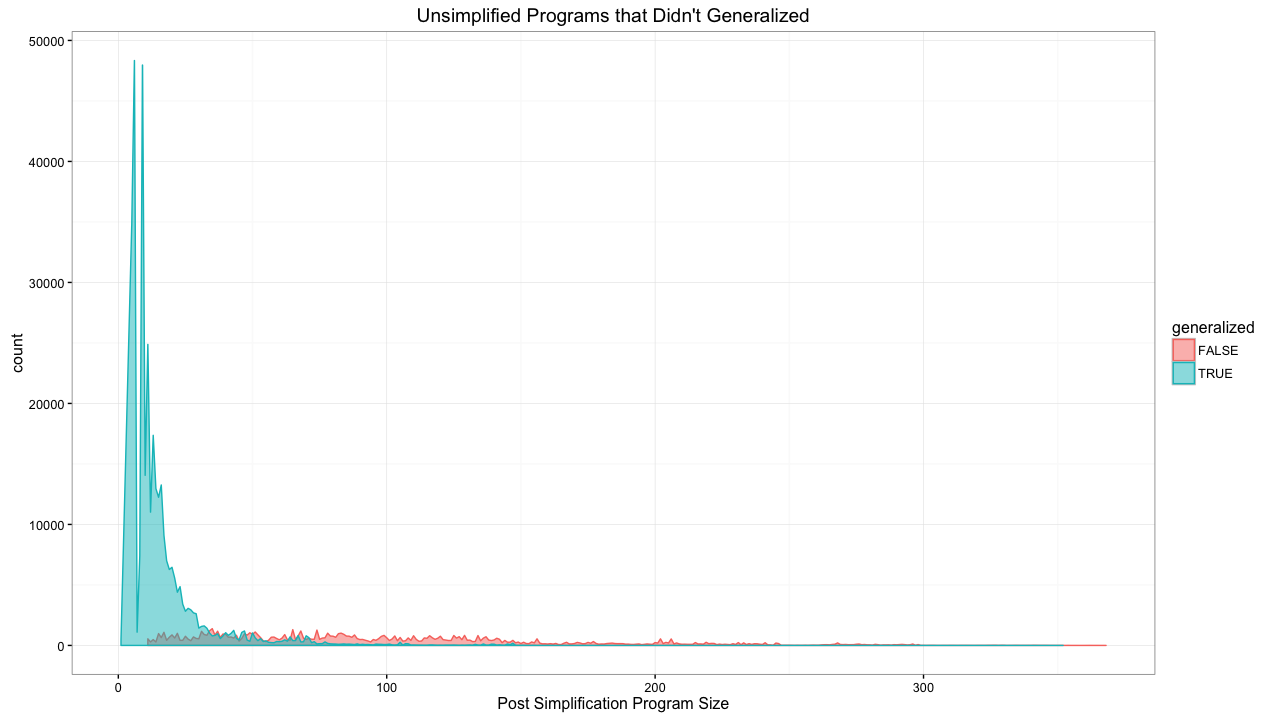
\includegraphics[width=\linewidth]{Size_density_by_generalized_count}
\caption{Size counts of simplified programs. Includes all simplified programs, from both ones that did and did not generalize pre-simplification.}
\label{fig:count:gen}
\end{figure}

\begin{figure}[t] %[t] sets the image at the top of the page; t = top, b = bottom, h = here%
\centering
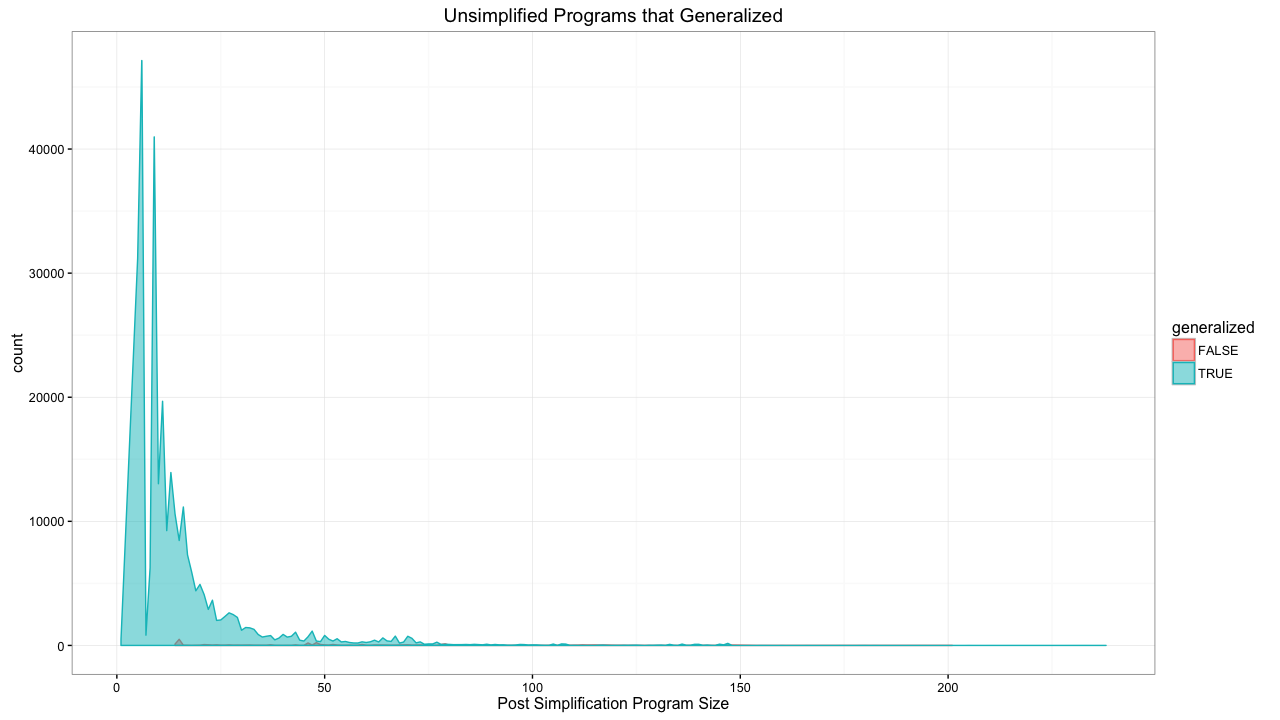
\includegraphics[width=\linewidth]{Size_density_by_generalized_A_no_facet_count}
\caption{Size counts of simplified programs where pre-simplified program did generalize.}
\label{fig:count:pre-simp-gen-true}
\end{figure}

\begin{figure}[t] %[t] sets the image at the top of the page; t = top, b = bottom, h = here%
\centering
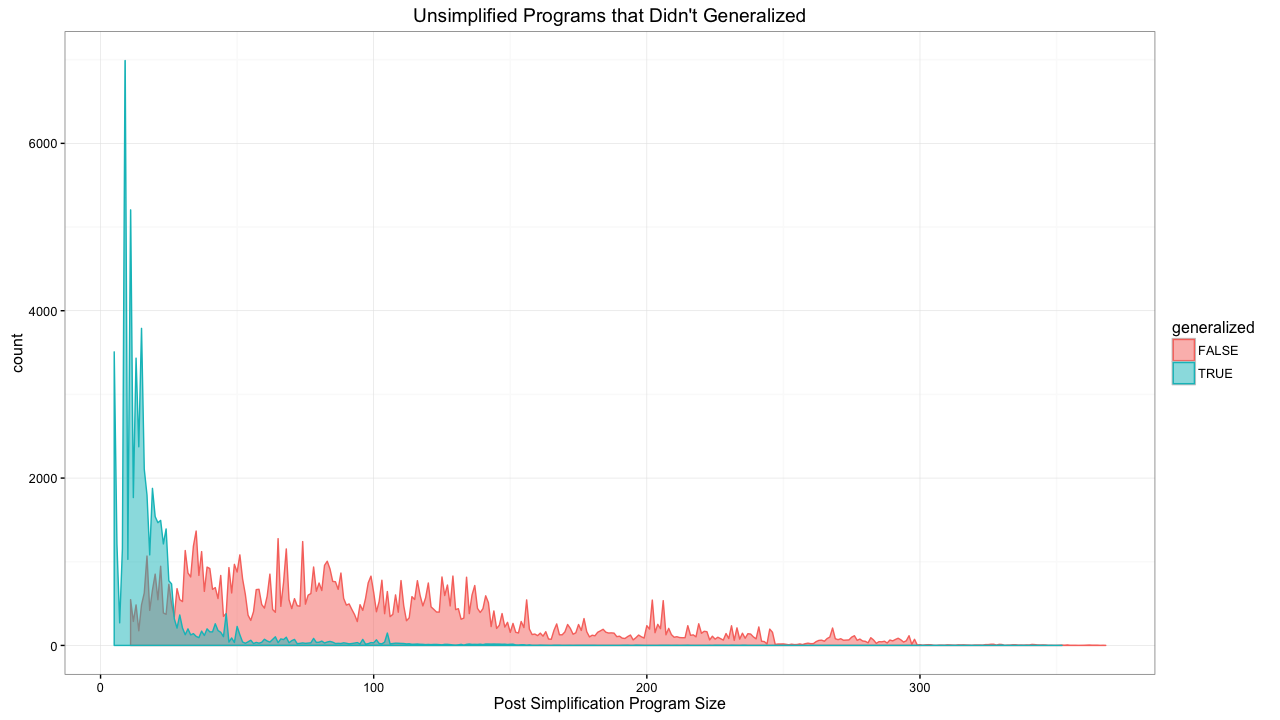
\includegraphics[width=\linewidth]{Size_density_by_generalized_B_no_facet_count}
\caption{Size counts of simplified programs where pre-simplified program did \underline{not} generalize.}
\label{fig:count:pre-simp-gen-true}
\end{figure}

These look at the same graphs, but faceted.

\begin{figure}[t] %[t] sets the image at the top of the page; t = top, b = bottom, h = here%
\centering
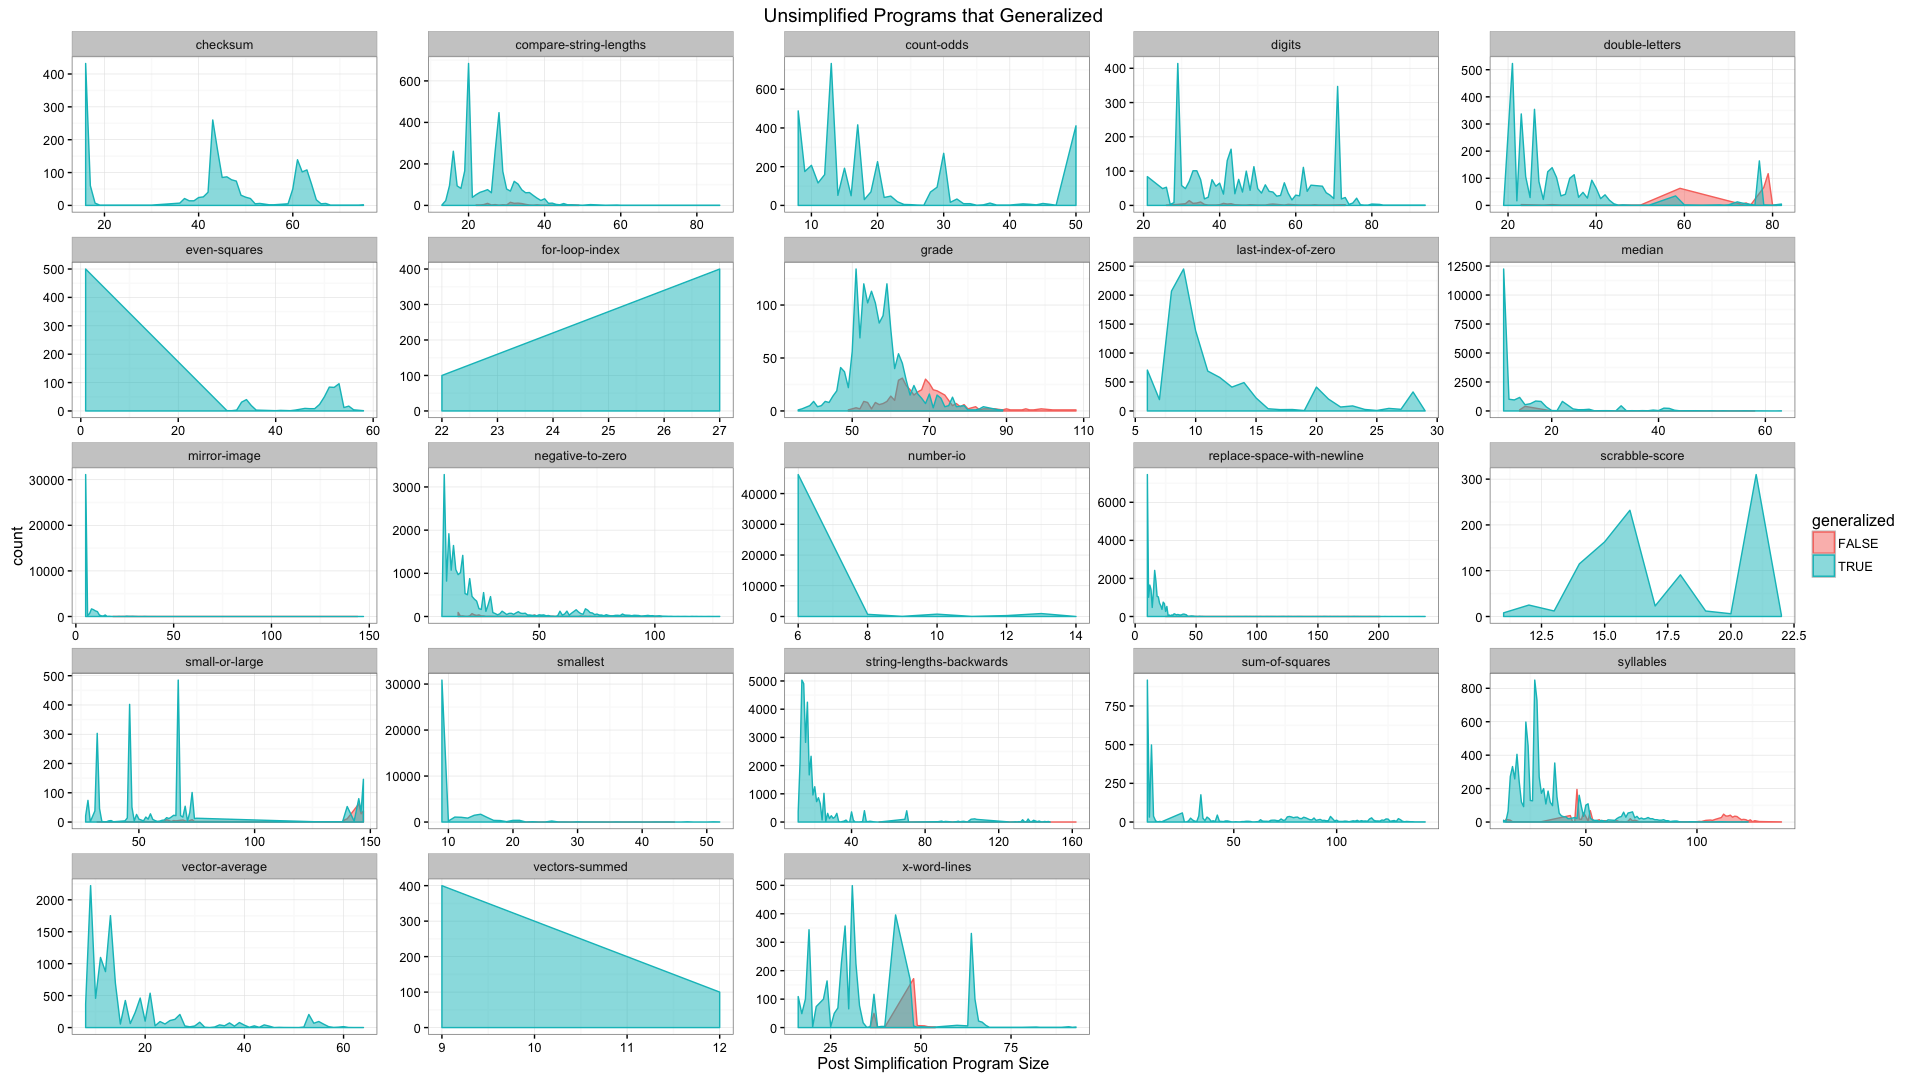
\includegraphics[width=\linewidth]{Size_density_by_generalized_A_count}
\caption{Size counts of simplified programs where pre-simplified program did generalize.}
\label{fig:count:pre-simp-gen-true}
\end{figure}

\begin{figure}[t] %[t] sets the image at the top of the page; t = top, b = bottom, h = here%
\centering
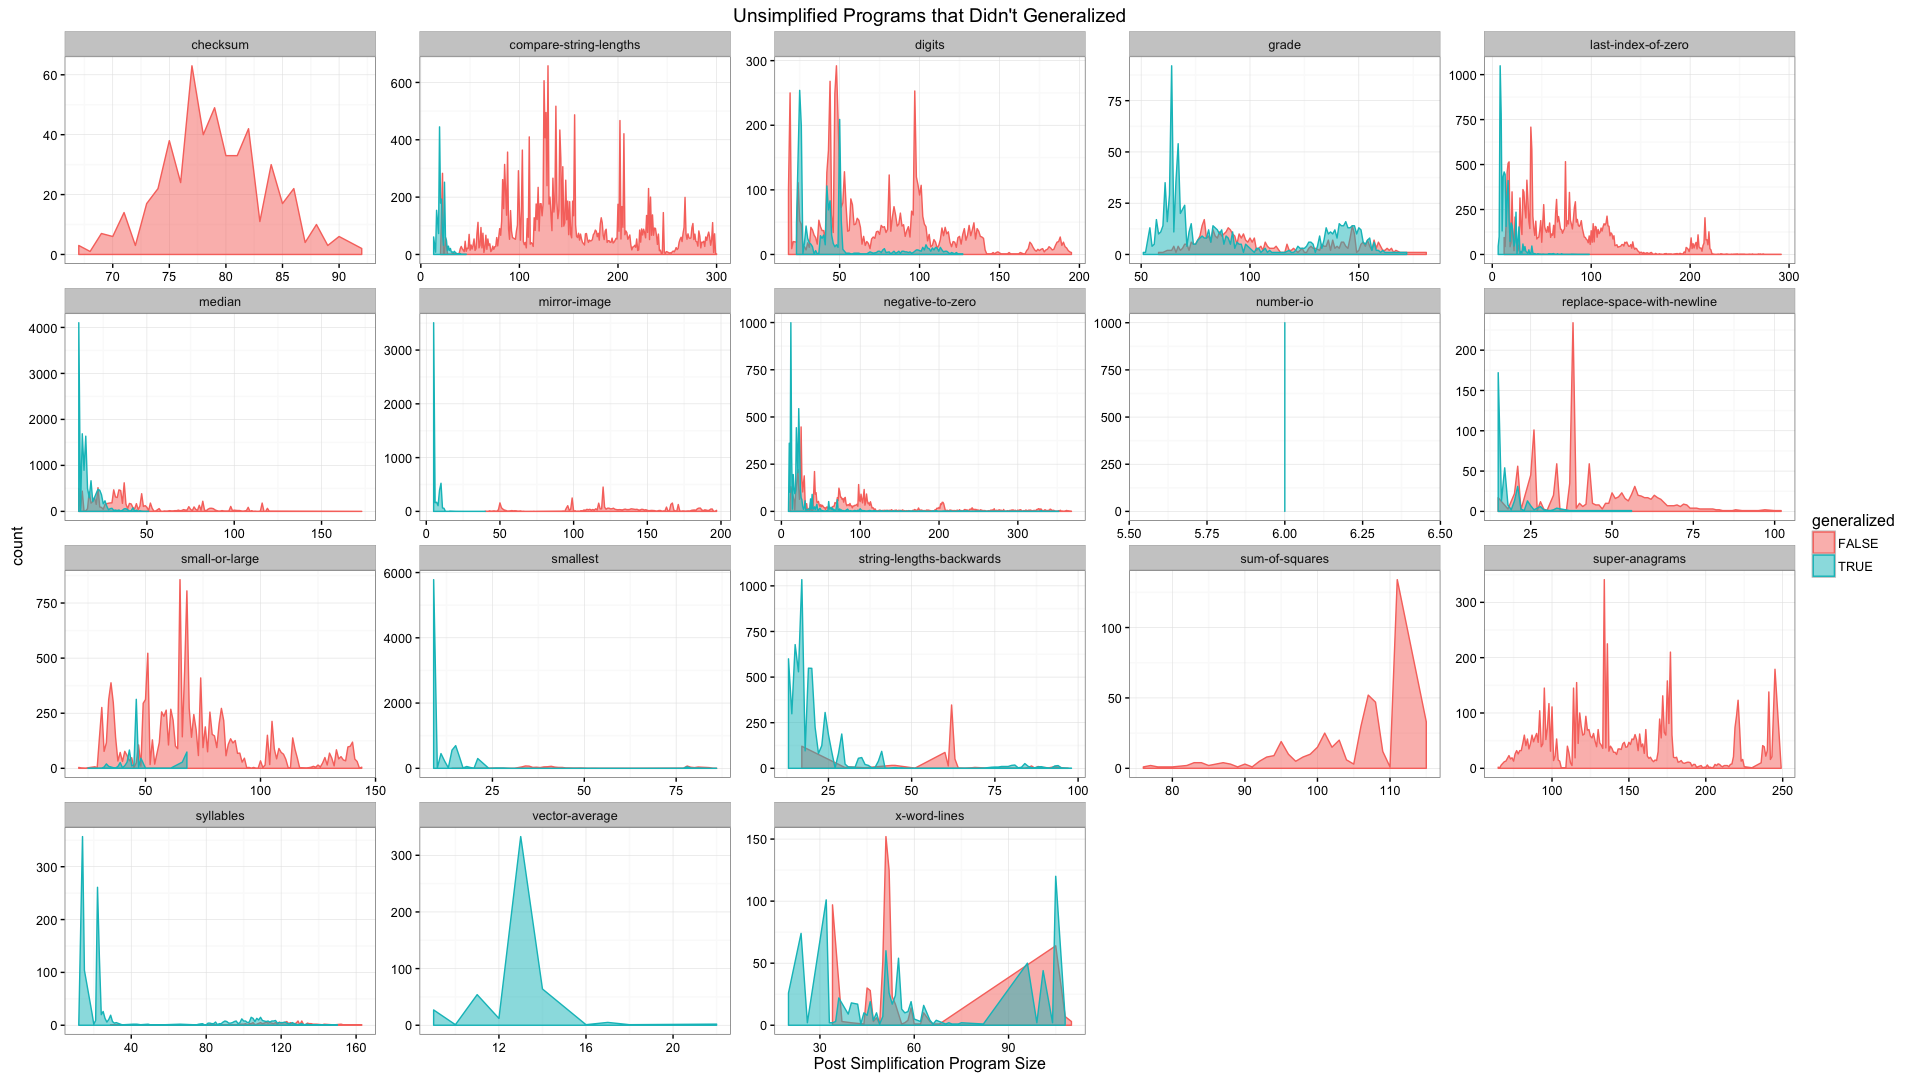
\includegraphics[width=\linewidth]{Size_density_by_generalized_B_count}
\caption{Size counts of simplified programs where pre-simplified program did \underline{not} generalize.}
\label{fig:count:pre-simp-gen-true}
\end{figure}

MORE FIGURES!

\begin{figure*}[t] %[t] sets the image at the top of the page; t = top, b = bottom, h = here%
\centering
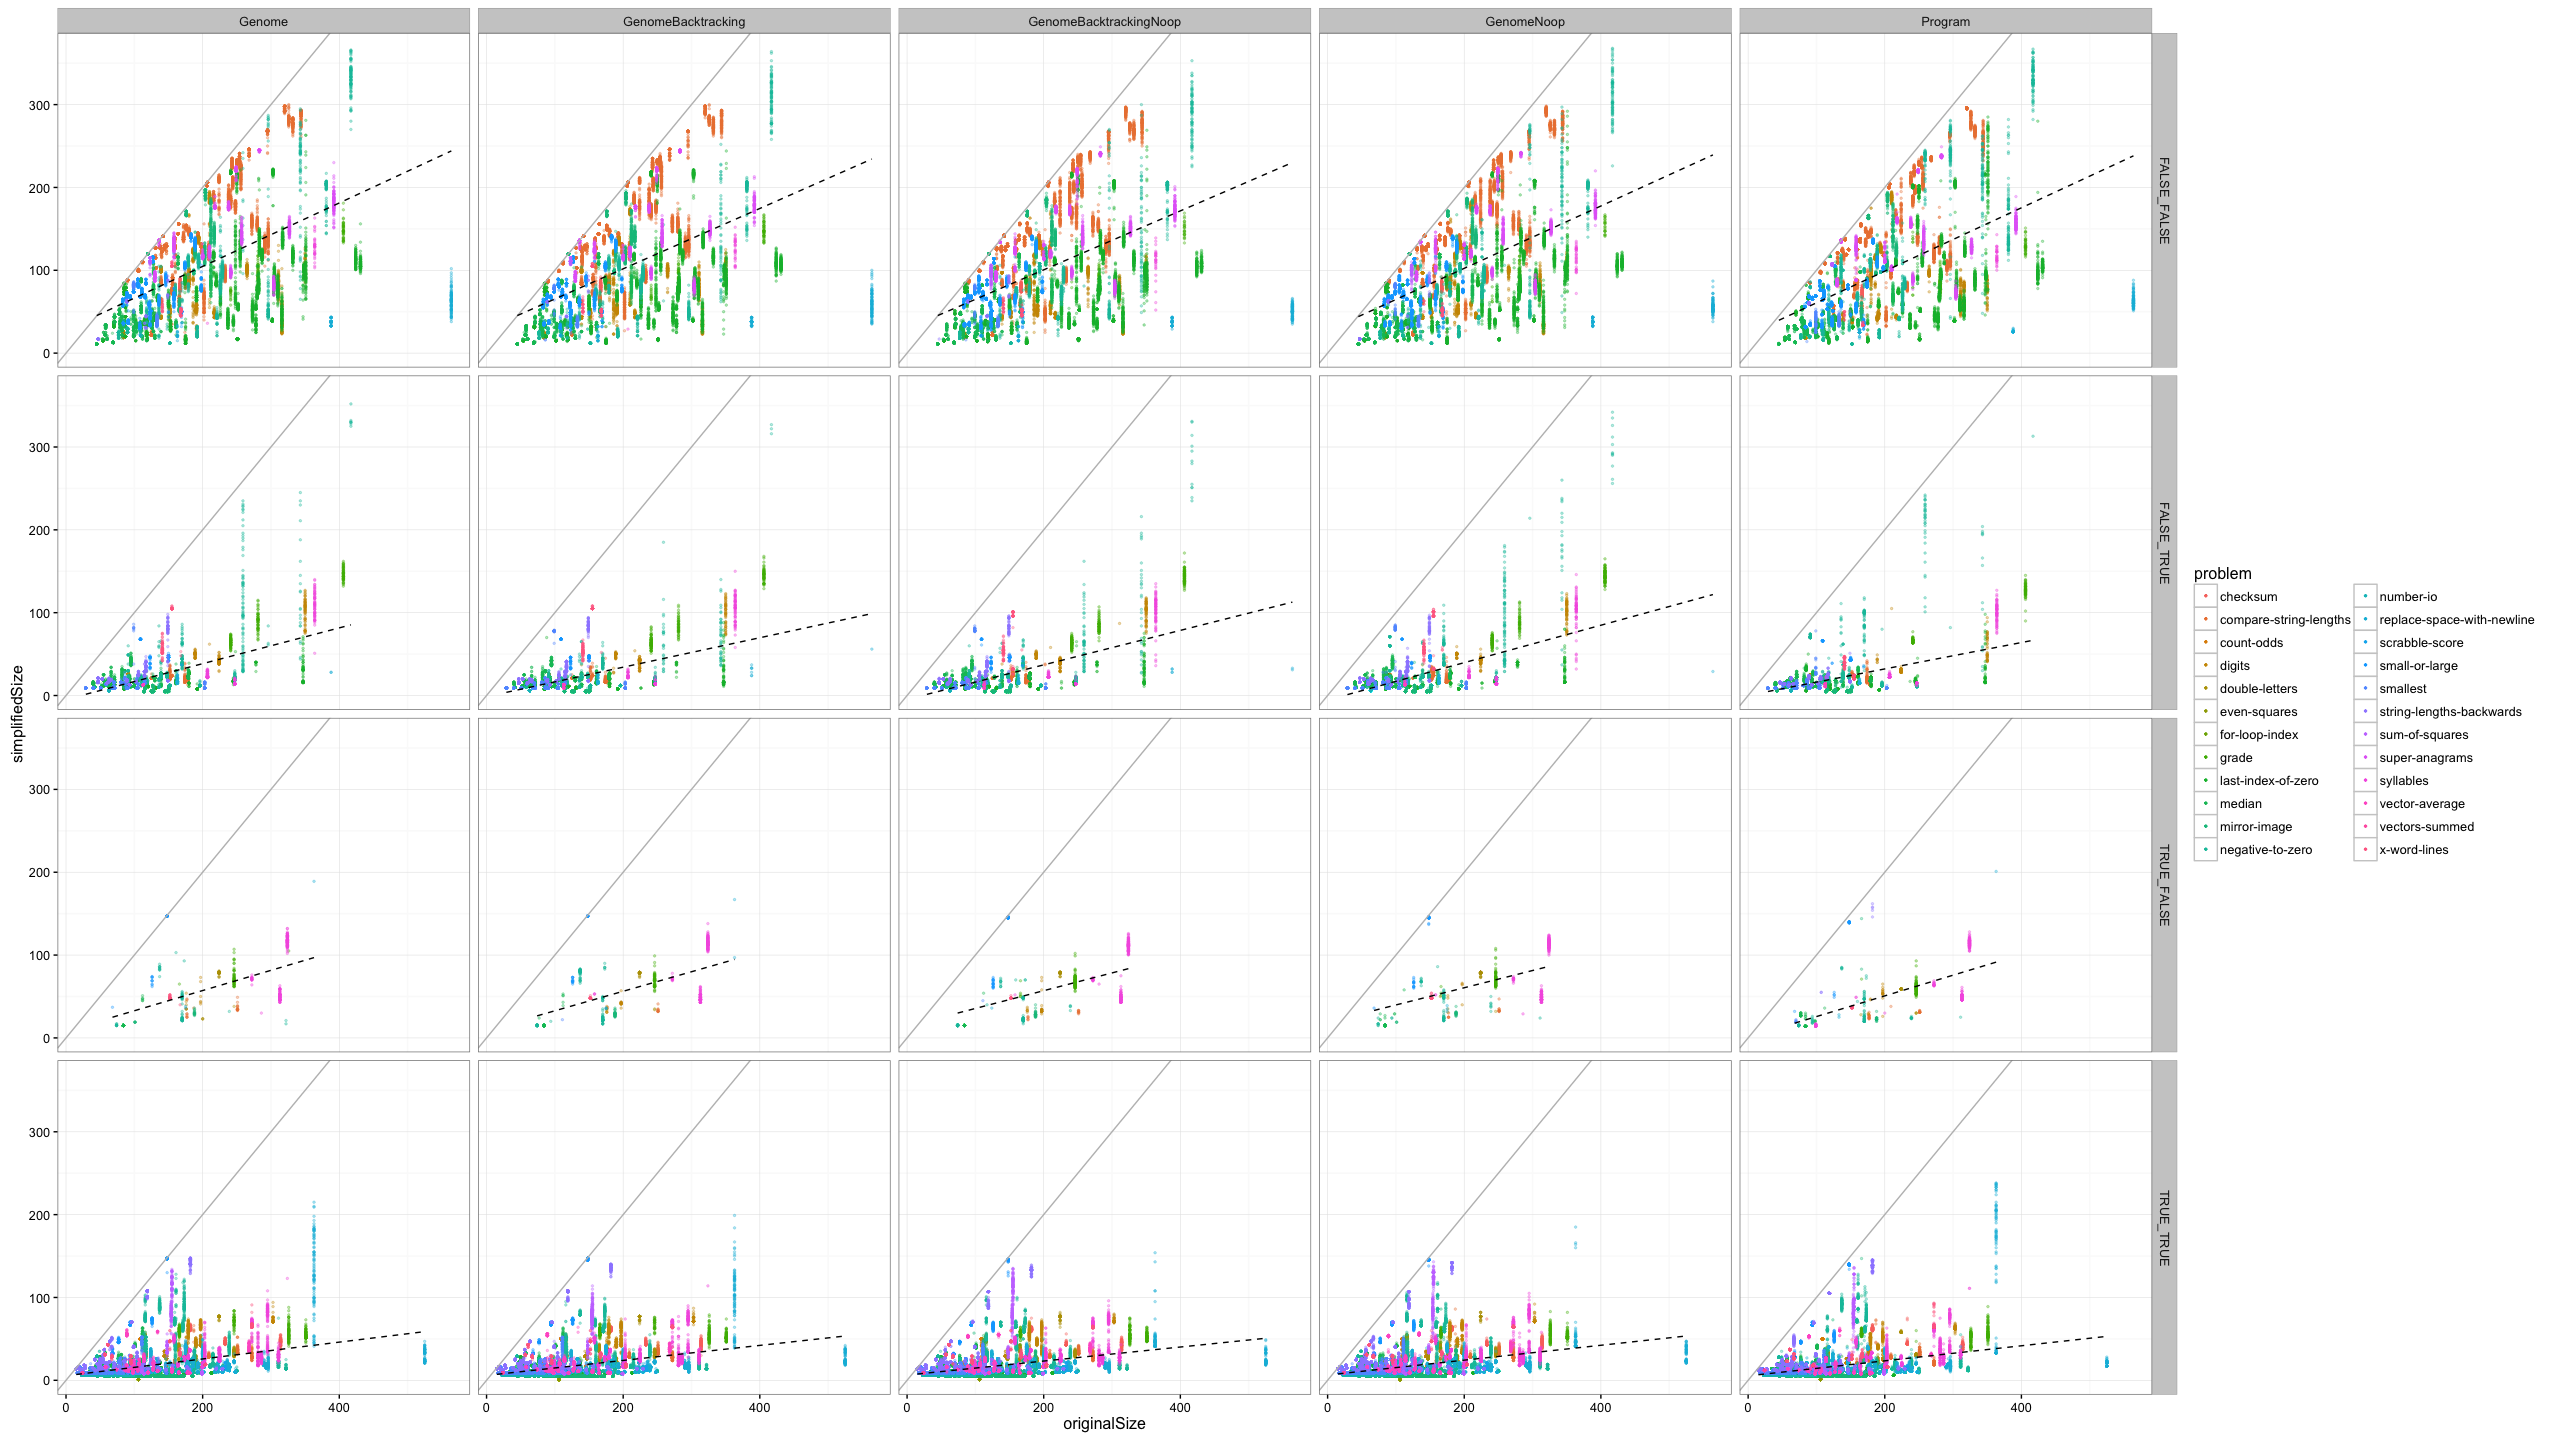
\includegraphics[width=\textwidth]{Nic_Plot_2} % \linewidth
\caption{[This figure is representative of 2 or 3 other similar figures that might fit these needs.] First row: pre- and post-simplification both didn't generalize. Second row: didn't generalize pre-simplification, then generalized post-simplification. Etc. The lines are linear fit lines. You can see that programs that generalized post-simplification have smaller slope on the trend lines!}
\label{fig:nic-plot}
\end{figure*}

\begin{figure*}[t] %[t] sets the image at the top of the page; t = top, b = bottom, h = here%
\centering
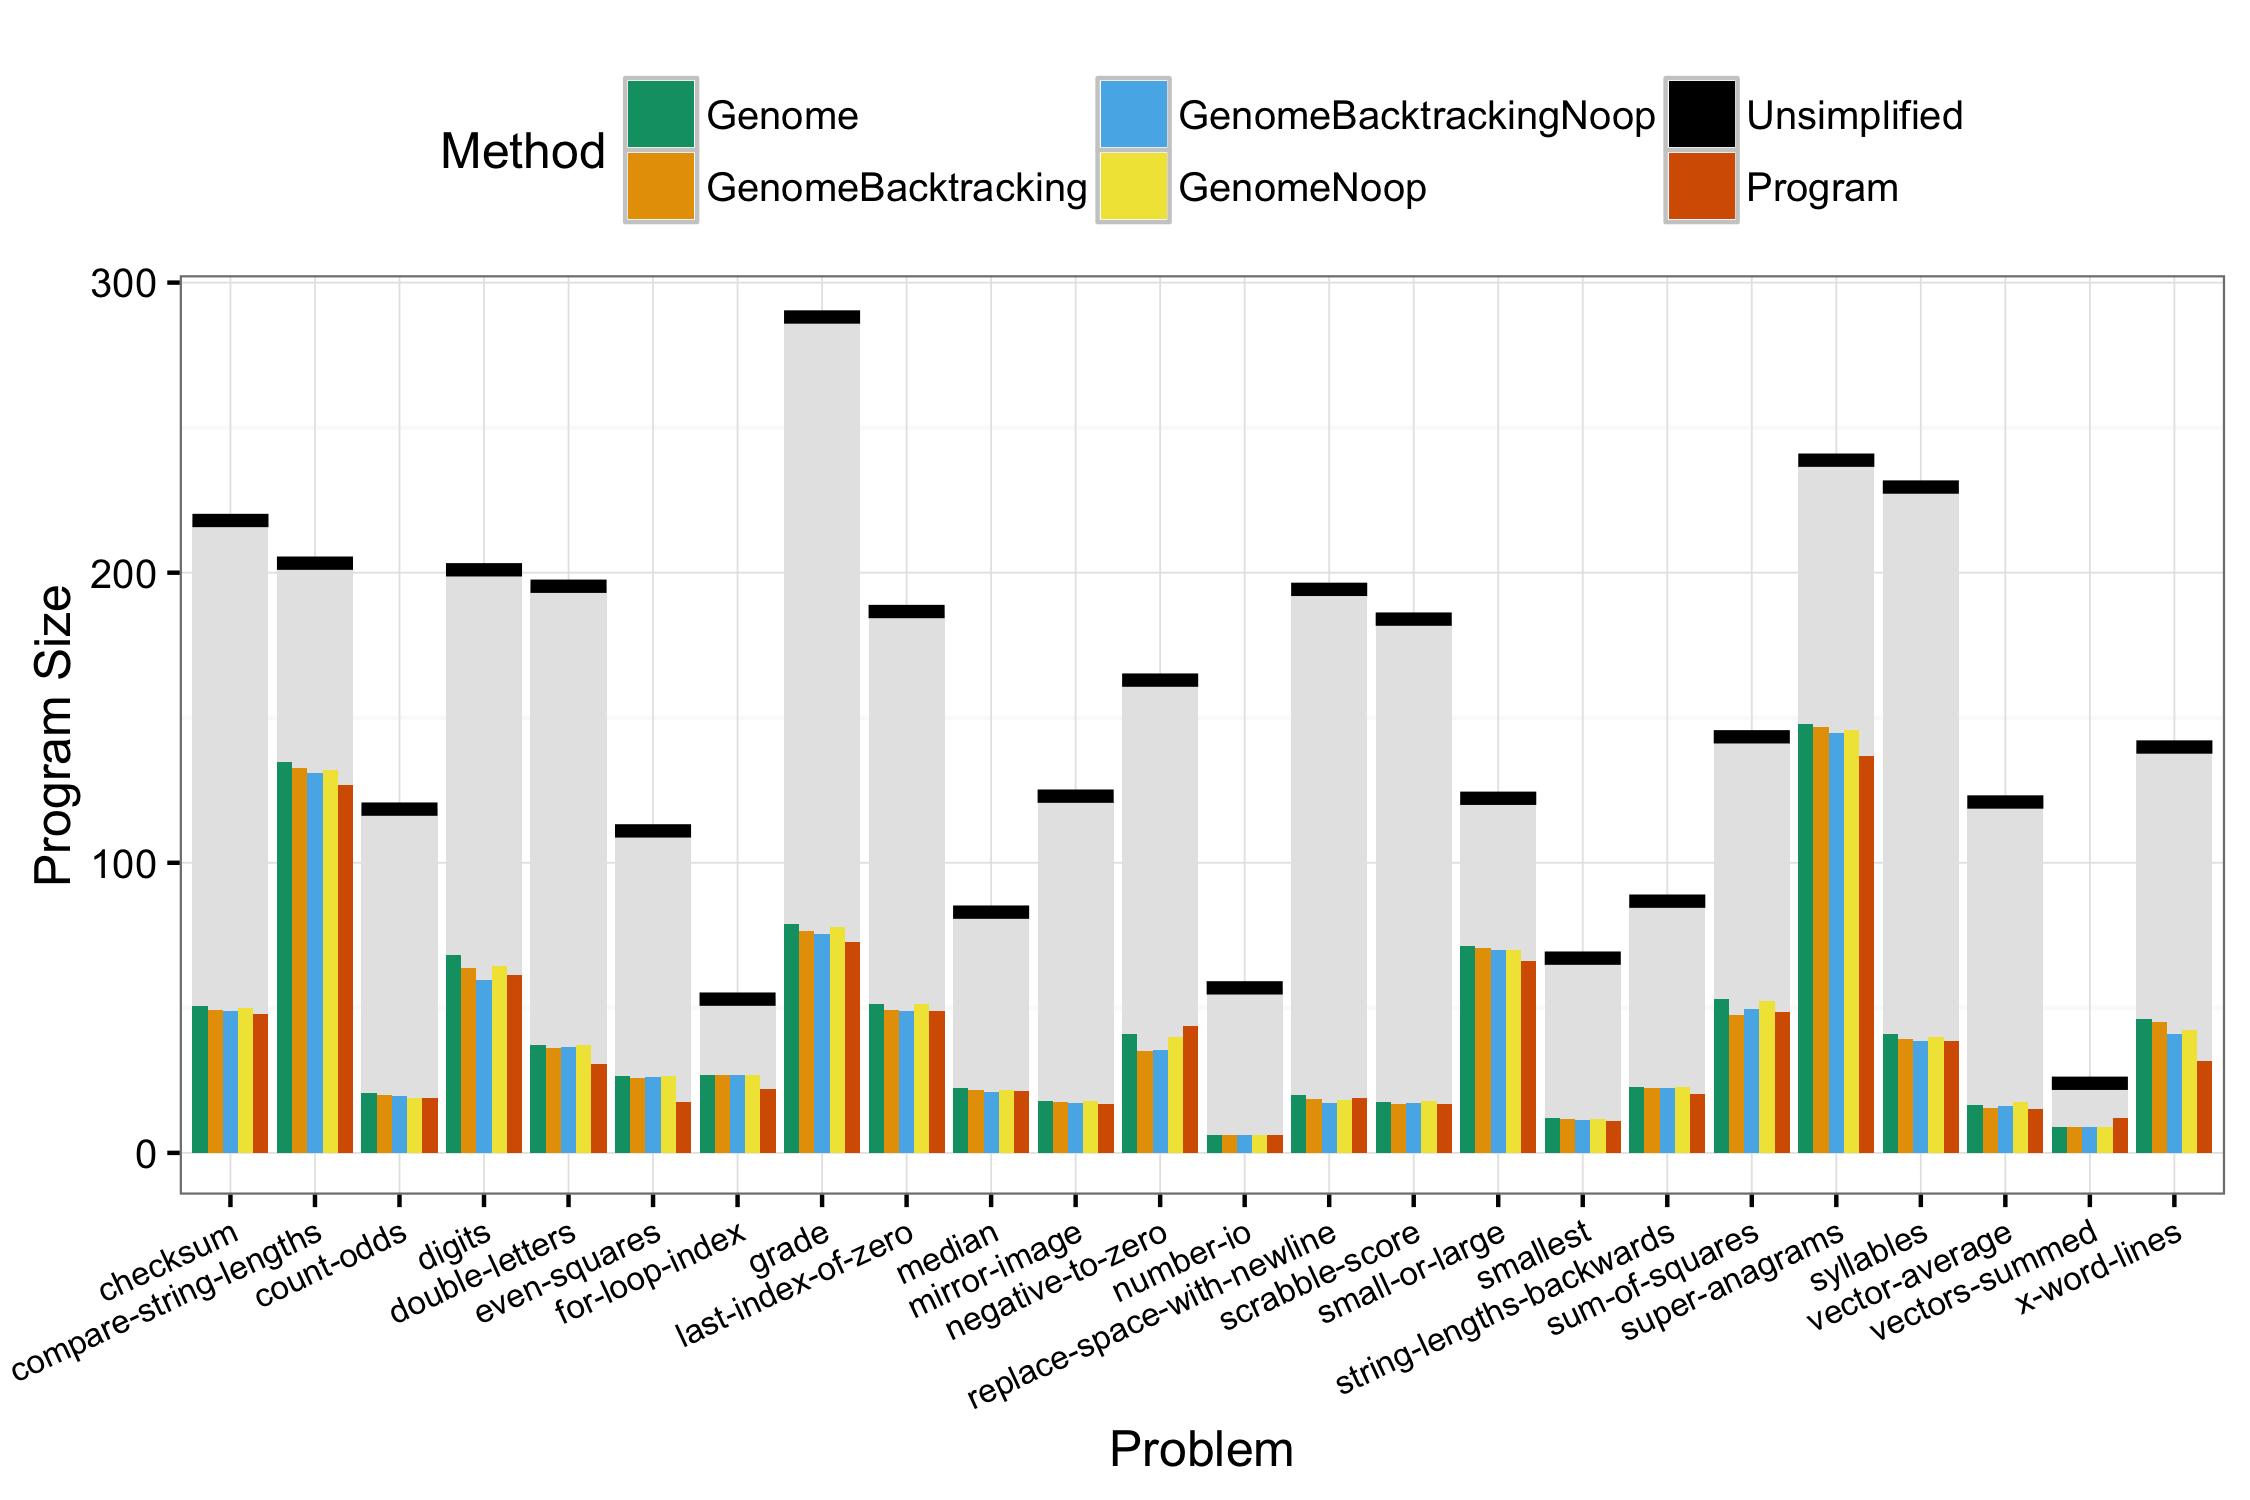
\includegraphics[width=\textwidth]{Problem_by_Size_bar} % \linewidth
\caption{For each method, the average program size of simplified programs.}
\label{fig:bar:size}
\end{figure*}

Question: In this figure, how much of the time are the simplified programs significantly better at generalization than the unsimplified programs? How would we measure this? Do we need to?

\begin{figure*}[t] %[t] sets the image at the top of the page; t = top, b = bottom, h = here%
\centering
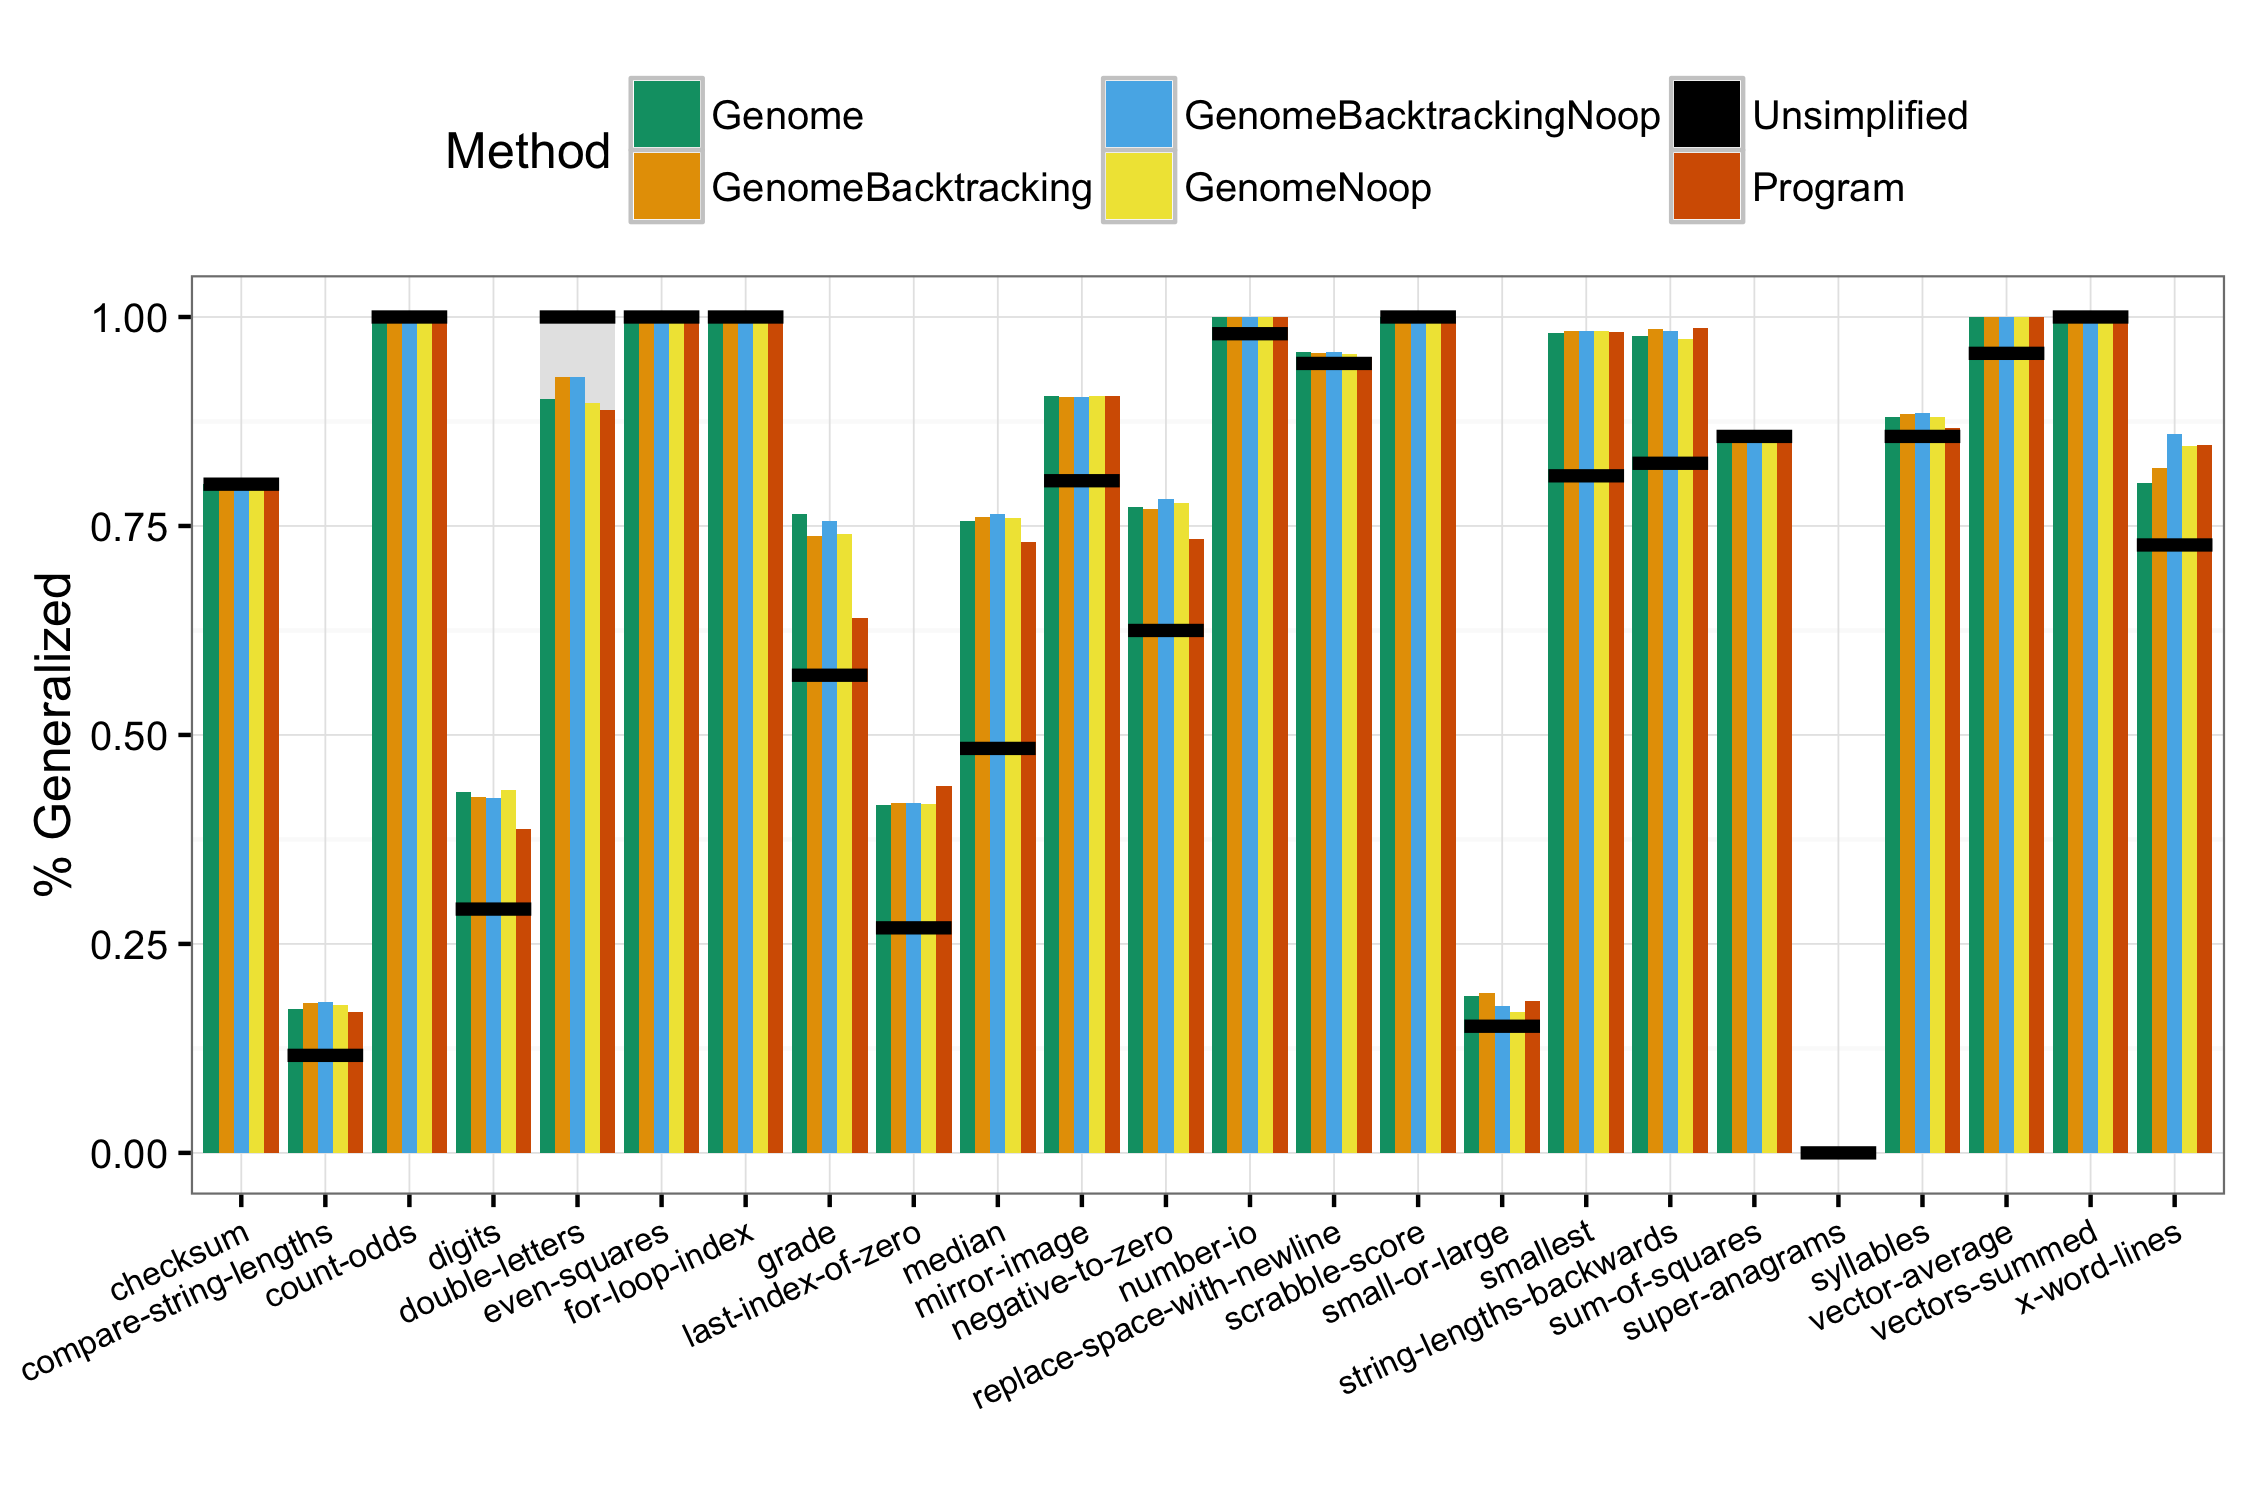
\includegraphics[width=\textwidth]{Problem_by_PcntGen_bar} % \linewidth
\caption{For each method, the percent of simplified programs that generalize to unseen data.}
\label{fig:bar:percent_generalization}
\end{figure*}

\begin{table}[t]
	\centering
	\caption{The average rank in generalization percent for each simplification variant, where lower rank means better generalization. This also includes the pre-simplification programs.}
	\label{table:generalization-ranks}
	\begin{tabu} to \textwidth {l r}
		\toprule
		\textbf{Variant} & \textbf{Average Rank} \\
		\midrule
		\textbf{Genome-Backtracking-Noop} & 2.73 \\
		\textbf{Genome-Backtracking} & 3.02 \\
		\textbf{Genome-Noop} & 3.29 \\
		\textbf{Genome} & 3.33 \\
		\textbf{Program} & 3.67 \\
		\textbf{Pre-Simplification} & 4.96 \\
		\bottomrule
	\end{tabu}
\end{table}

\begin{table}[ht]
	\centering
	\caption{The average rank in size for each simplification variant, where lower rank means smaller programs. This also includes the pre-simplification programs. Note the different order of methods from Table~\ref{table:generalization-ranks}.}
	\label{table:size-ranks}
	\begin{tabu} to \textwidth {l r}
		\toprule
		\textbf{Variant} & \textbf{Average Rank} \\
		\midrule
		\textbf{Program} & 1.87 \\
		\textbf{Genome-Backtracking-Noop} & 2.12 \\
		\textbf{Genome-Backtracking} & 2.79 \\
		\textbf{Genome-Noop} & 3.60 \\
		\textbf{Genome} & 4.60 \\
		\textbf{Pre-Simplification} & 6.00 \\
		\bottomrule
	\end{tabu}
\end{table}

\section{Discussion}
\label{sec:discussion}

\todo[inline]{Talk about what the results mean}

Here are some potentially interesting questions to explore with this data:

    Which simplification method tends to result in the smallest programs on average? Is there any significant differences here?

    Is getting smaller during simplification important for generalization? In other words, do smaller programs post-simplification tend to generalize better than larger ones?

        Note: we could ask this question of all the simplified programs, but we could also concentrate only on runs that had some generalizing programs and some non-generalizing programs, which might give us a more detailed view. It would probably be worthwhile to look into both of these. I'm not sure exactly how we would investigate this. @mcphee made some cool graphs last year that start answering this question. I've included one at the bottom of this post that was made with limited data; a similar graph for the full data might be a good place to start.

    It might be worthwhile to break this big plot into smaller plots, grouping together similar plots. For example, we might group plots based on how often unsimplified programs generalize -- groups of something like 0-50\%, 50-95\%, and 95-100\% generalization. Or, we could do it some other way. But, this could definitely help with spotting differences based on problem.

    Would a multi-restart simplification get us to smaller programs more often than the other methods we've tried? This could potentially avoid unlucky local minima. The backtracking methods are also trying to avoid unlucky local minima, so this would be an interesting comparison. It seems like we could answer this question with the data we have.




\section{Related Work}
\label{sec:related}

\todo[inline]{Tom: I'm fine moving this section earlier if others prefer.}

\todo[inline]{Below are things I've (Tom) come across in the past year potentially realted to this work. We'll have to go through and see what's worth citing.}

\subsection{Papers about automatic simplification}

\begin{itemize}

\item
Genprog minimization after run (see 7/24/16)

\item
Field Guide to Genetic Programming: p 64 top: Bahnzaf paper might be precursor to automatic simplification

\item
This paper in neural networks might be related: GECCO 2016 - Identifying Core Functional Networks and Functional Modules within Artificial Neural Networks via Subsets Regression

\item
Differentiate between our work and algebraic simplification (as used in semantic GP), since this CAN change the semantics on inputs not in the training set, where algebraic methods cannot. Also, algebraic methods wouldn't work on general programs that we're evolving

\item
Algebraic Simplification of GP Programs During Evolution (I think this is an actual paper title)

\item
Investigation of simplification threshold and noise level of input data in numerical simplification of genetic programs \cite{Kinzett:2010:cec}

\item
Smaller networks in neural nets: https://push-language.hampshire.edu/t/gecco-2017-simplification-for-generalization/660/21?u=thelmuth

\end{itemize}

\subsection{Papers about generalization and overfitting in GP}

\begin{itemize}
\item
GECCO 2011 - Variance based Selection to Improve Test Set Performance in Genetic Programming

\item
Controlling overfitting in symbolic regression based on a bias/variance error decomposition


\end{itemize}

\subsection{Other related papers}

\begin{itemize}
\item
Tree-structured differencing: R. Al-Ekram, A. Adma, and O. Baysal. diffX: an algorithm to detect changes in multi-version XML documents. In Conference of the Centre for Advanced Studies on Collaborative research, pages 1–11. IBM Press, 2005.

\item
Delta debugging: A. Zeller. Yesterday, my program worked. Today, it does not. Why? In Foundations of Software Engineering, pages 253–267, 1999.

\end{itemize}

\section{Conclusions and future work}
\label{sec:conclusions}

\todo[inline]{Maybe this could/should be two sections, but I bet we won't have room.}

\begin{acks}
  
  \todo[inline]{Put acknowledgements here, including grants.}

\end{acks}
